%!TEX root = principal.tex
\section{Redes de Comunicação: Introdução e noções básicas}
Na pirâmide de automação, a partir da camada 2, os sistemas utilizados são softwares em computadores, sejam servidores, terminais, desktops, notebooks ou mesmo tablets e smartphones (para o caso do supervisório). No nível de controle, o dispositivo utilizado pode ser um computador, um CLP -- que não deixa de ser um computador -- ou outro dispositivo que incorpora um processador. Hoje em dia até no nível 0 estão ficando cada vez mais comuns os dispositivos ditos \emph{inteligentes}, que incorporam também um microprocessador. A comunicação entre eles é feita por uma rede de dados, tais como a ethernet.

O problema da comunicação de dados automática entre diversos dispositivos é bastante complexo. Ele envolve a:
\begin{enumerate}
	\item transferência de dados de um dispositivo a outro,
	\item em alta velocidade,
	\item sem perda de informação,
	\item eventualmente passando por dispositivos intermediários,
	\item talvez envolvendo sistemas de comunicação diferentes,
	\item com privacidade,
	\item sem envolver outros dispositivos desnecessariamente.
\end{enumerate}

Peguemos como exemplo pagar uma conta via internet. Logo é neceesária a comunicação do dispositivo caseiro (que seja um tablet) e o computador central do banco (1). Quanto mais rápida for esta comunicação, mais agradável é para o usuário e mais barato é para o banco (2). Obviamente nenhuma das partes envolvidas querem que seja pago o valor errado ou a conta errada (3). Entre o tablet e o servidor do banco estão: o modem wifi, a central telefônica, servidores da companhia telefônica e talvez de outras fornecedoras de serviço (4), e em geral não é do interesse do usuário que a companhia telefônica ou outro elemento saiba de sua senha do banco (6). A comunicação do tablet ao modem é por wifi. Do modem para a central telefônica é pelo fio telefônico. Da central em diante pode ser por cabos de cobre ou, mais provavelmente, por fibra óptica (5). Também, por questão de custos e privacidade, não é desejável que outros elementos recebam aquela informação, mesmo que criptografada.

Para resolver este problema, foi desenvolvida a idéia de quebrá-lo em várias partes, ou camadas, onde cada camada é responsável por uma determinada parte do problema. A informação fica então passando de camada a camada para resolver todas as questões relativas à comunicação. Tal esquema é também chamado de pilha de protocolos.

\subsection{Modelo OSI}
Diferentes tipos de rede de dados tem problemas diferentes. O modelo OSI procura definir camadas o mais genéricas possíveis, de modo a abarcar qualquer tipo de comunicação de dados. Este modelo define 7 camadas: física, enlace, rede, transporte, sessão, apresentação e aplicação.

\subsubsection{Física}
	A camada física é a única que não pode ser implementada em software. Ela lida com as definições eletro-mecânicas necessárias para a comunicação. Ou seja, a camada física define:
	\begin{itemize}
		\item a forma como os dados são transmitidos (sinais elétricos por cabo, sinais de rádio, luz, etc);
		\item as características do meio de transmissão, tais como o tipo de cabo, os níveis de tensão, o formato dos conectores, etc;
		\item a taxa de transmissão.
	\end{itemize}
	Note-se que a taxa de transmissão acaba sendo limitada justamente pelos diversos parâmetros físicos descritos pela camada física de um determinado protocolo de comunicação.

Outro parâmetro definido na camada física é se a rede é \emph{simplex}, \emph{half-duplex} ou \emph{full-duplex}. Simplex significa que a comunicação no meio de transmissão é apenas num sentido (exemplo: televisão), half-duplex é uma comunicação em dois sentidos, mas apenas um por vez (exemplo: walkie-talkie) e full-duplex é uma comunicação em ambos os sentidos ao mesmo tempo (exemplo: telefonia).

\subsubsection{Enlace}

A camada de enlace cuida da comunicação de um dispositivo a seu vizinho, que não necessariamente são os pontos finais.

No exemplo acima, esta seria a comunicação entre o tablet e o modem wifi; entre o modem e a central; entre a central e o servidor da companhia telefônica, e assim por diante.

A camada de enlace de um protocolo define quem acessa o meio de transmissão e quando, que sinais indicam o início e o fim de uma transmissão, mecanismos que detectem e/ou corrijam erros e, se necessário, para qual dentre vários dispositivos é aquela comunicação específica.

Alguns protocolos de comunicação, tais como USB e ethernet, fazem a conexão ponto a ponto. Neste caso apenas 2 dipositivos podem acessar o meio. Outros sistemas, como o wifi, podem ter vários (em alguns casos, centenas) de dispositivos no mesmo meio. O que torna necessário a definição de quem pode acessar o meio em cada instante. Várias possibilidades existem:
\begin{description}
	\item[mestre-escravo] Neste sistema, a comunicação sempre é iniciada pelo mestre, e um escravo só ocupa o meio quando o mestre requisita uma informação. Ex.: USB, Modbus.
	\item[\emph{token ring}] É passada uma ficha (token) virtual entre os dispositivos. Quem tem a ficha pode falar.
	\item[Multiplexação por tempo] Cada dispositivo tem uma hora específica para controlar o barramento. Um sinal periódico (NUT- \emph{Network Update Time}) sincroniza os dispositivos.
	\item[CSMA-CD -- \emph{Carrier Sense Multiple Access with Collision Detection}] Sempre que um dispositivo quer se comunicar com outro, ele checa antes se o meio está livre. Ex.: wi-fi, bluetooth, CAN.
\end{description}

Tipicamente os protocolos da camada de enlace acrescentam uma certa redundância ao dado transmitido, o que permite detectar e até corrigir erros de transmissão. São os chamados códigos corretores de erro, dentre os quais se utiliza bastante o CRC - \emph{Cyclic Redundancy Check}.

\subsubsection{Rede}
Camada responsável pelo roteamento da informação. Ou seja: Se A quer se comunicar com D, mas A apenas tem ligação direta com B e C, para quem A deve mandar a informação?

Tipicamente este roteamento é feito através de uma tabela que mapeia o endereço lógico de um dispositivo (o endereço usado nas etapas acima, tais como o IP) e o endereço físico, usado pela camada de enlace (muitos sistemas usam o \emph{MAC address}). Esta é a última camada a que uma comunicação chega num dispositivo que não o inicial ou final: o programa desta camada checa se o endereço lógico da mensagem é o mesmo daquele dispositivo; não sendo, ele busca na tabela qual o endereço físico para o qual reenviar aquela mensagem e reenvia, tal qual mostra a figura \ref{fig:camada_rede}. Isto serve também para fazer a conexão entre diferentes redes.

\begin{figure}[hbt]
	\begin{center}
		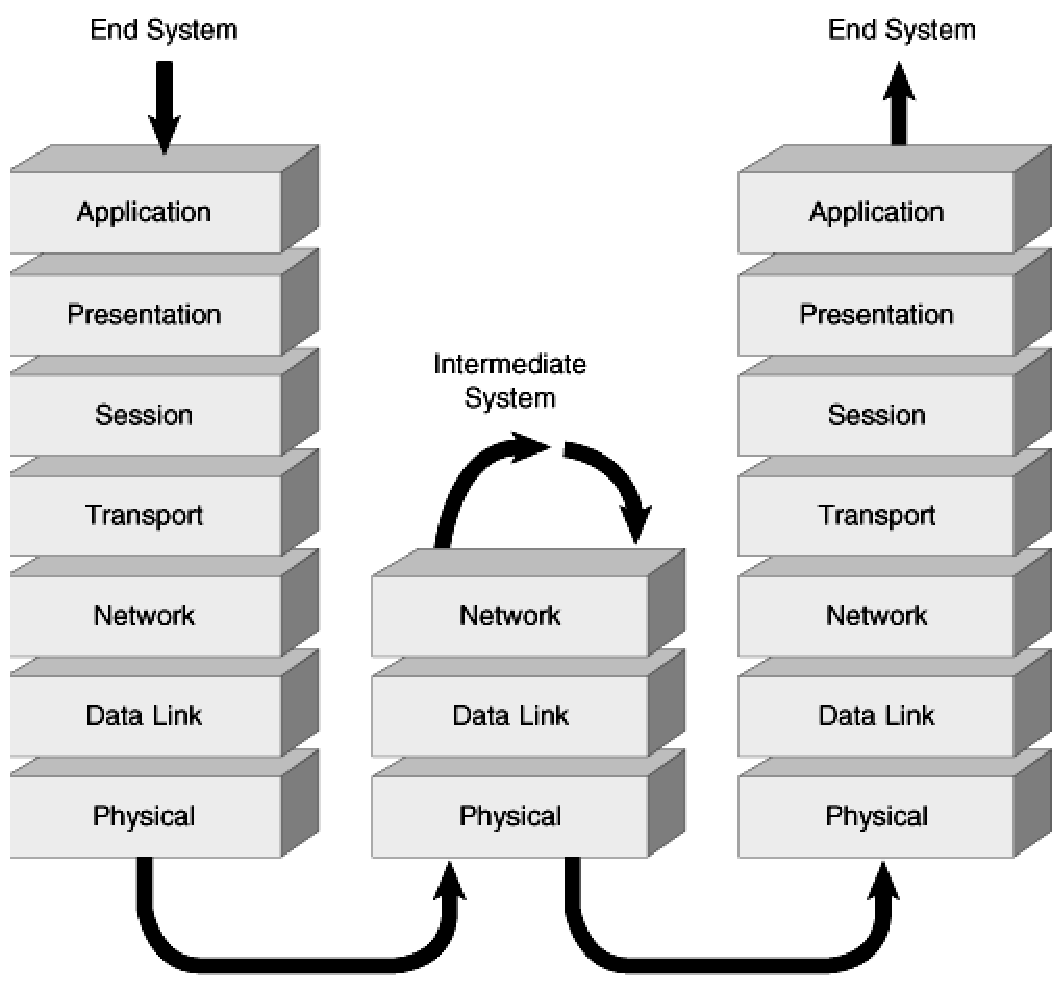
\includegraphics[width=0.6\textwidth]{figuras/network_layer}
	\end{center}
	\caption{Comunicação passando por dispositivo intermediário.}
	\label{fig:camada_rede}
\end{figure}

\subsubsection{Transporte}
 A camada de transporte cuida da comunicação entre o ponto inicial e final. Usa apenas o endereço lógico.
 Esta camada pode resolver quebrar uma mensagem grande em vários pacotes, mandando um pacote de cada vez para a camada de rede e remontando a mensagem no recebimento.

 Um conceito interessante utilizado na camada de transporte é o de \emph{Quality of Service -- QoS}, qualidade de serviço. Um sistema com alto QoS garante a chegada de todos os pacotes, na ordem em que foram enviados.

 A internet foi originalmente pensada como um sistema de baixo QoS, voltado para a trasnmissão de arquivos. A ordem dos pacotes não interessa e nem o atraso de um pacote. Caso um pacote se perca, simplesmente pede-se que seja reenviado. Uma rede de telefonia, por outro lado, busca garantir que o tempo de cada pacote seja o mesmo, para não piorar a qualidade da voz transmitida.

 Para diversas aplicações industriais, o QoS é importante: não se pode aceitar que uma mensagem de alarme, por exemplo, demore muito a chegar. EtherCAT - \emph{Ethernet for Control Automation Technology} é uma modificação de Ethernet para mensagens com diferentes QoS.
\subsubsection{Sessão}
Esta camada cria, gerencia e termina conexões entre 2 pontos de uma rede. É mais comum na telefonia, onde se gera um caminho fixo para uma determinada ligação. Basicamente esta camada gera a tabela que é usada pela camada de rede.
\subsubsection{Apresentação}
Faz a mudança no formato dos dados. Exemplo: troca de quebra de linha entre sistemas Unix e Windows, mudança de codificação windows 1252 para UTF, etc.

Inclue também a criptografia, que é a base para garantir a privaciade da comunicação ponto-a-ponto.
\subsubsection{Aplicação}
A aplicação final
\subsection{Internet}
	A Internet define uma pilha de apenas 4 protocolos: o de enlace, que engloba também o físico; o IP -- \emph{Internet Protocol}, equivalente ao de rede do modelo OSI; o de transporte, que pode ser um entre vários, sendo o TCP e o UDP os mais comuns e o de aplicação, que envolve sessão, apresentação e aplicação num só.

	A figura \ref{fig:tcp-ip} mostra a sequência que é feita com uma informação passada por http pela internet.
	\begin{figure}[hbt]
		\begin{center}
			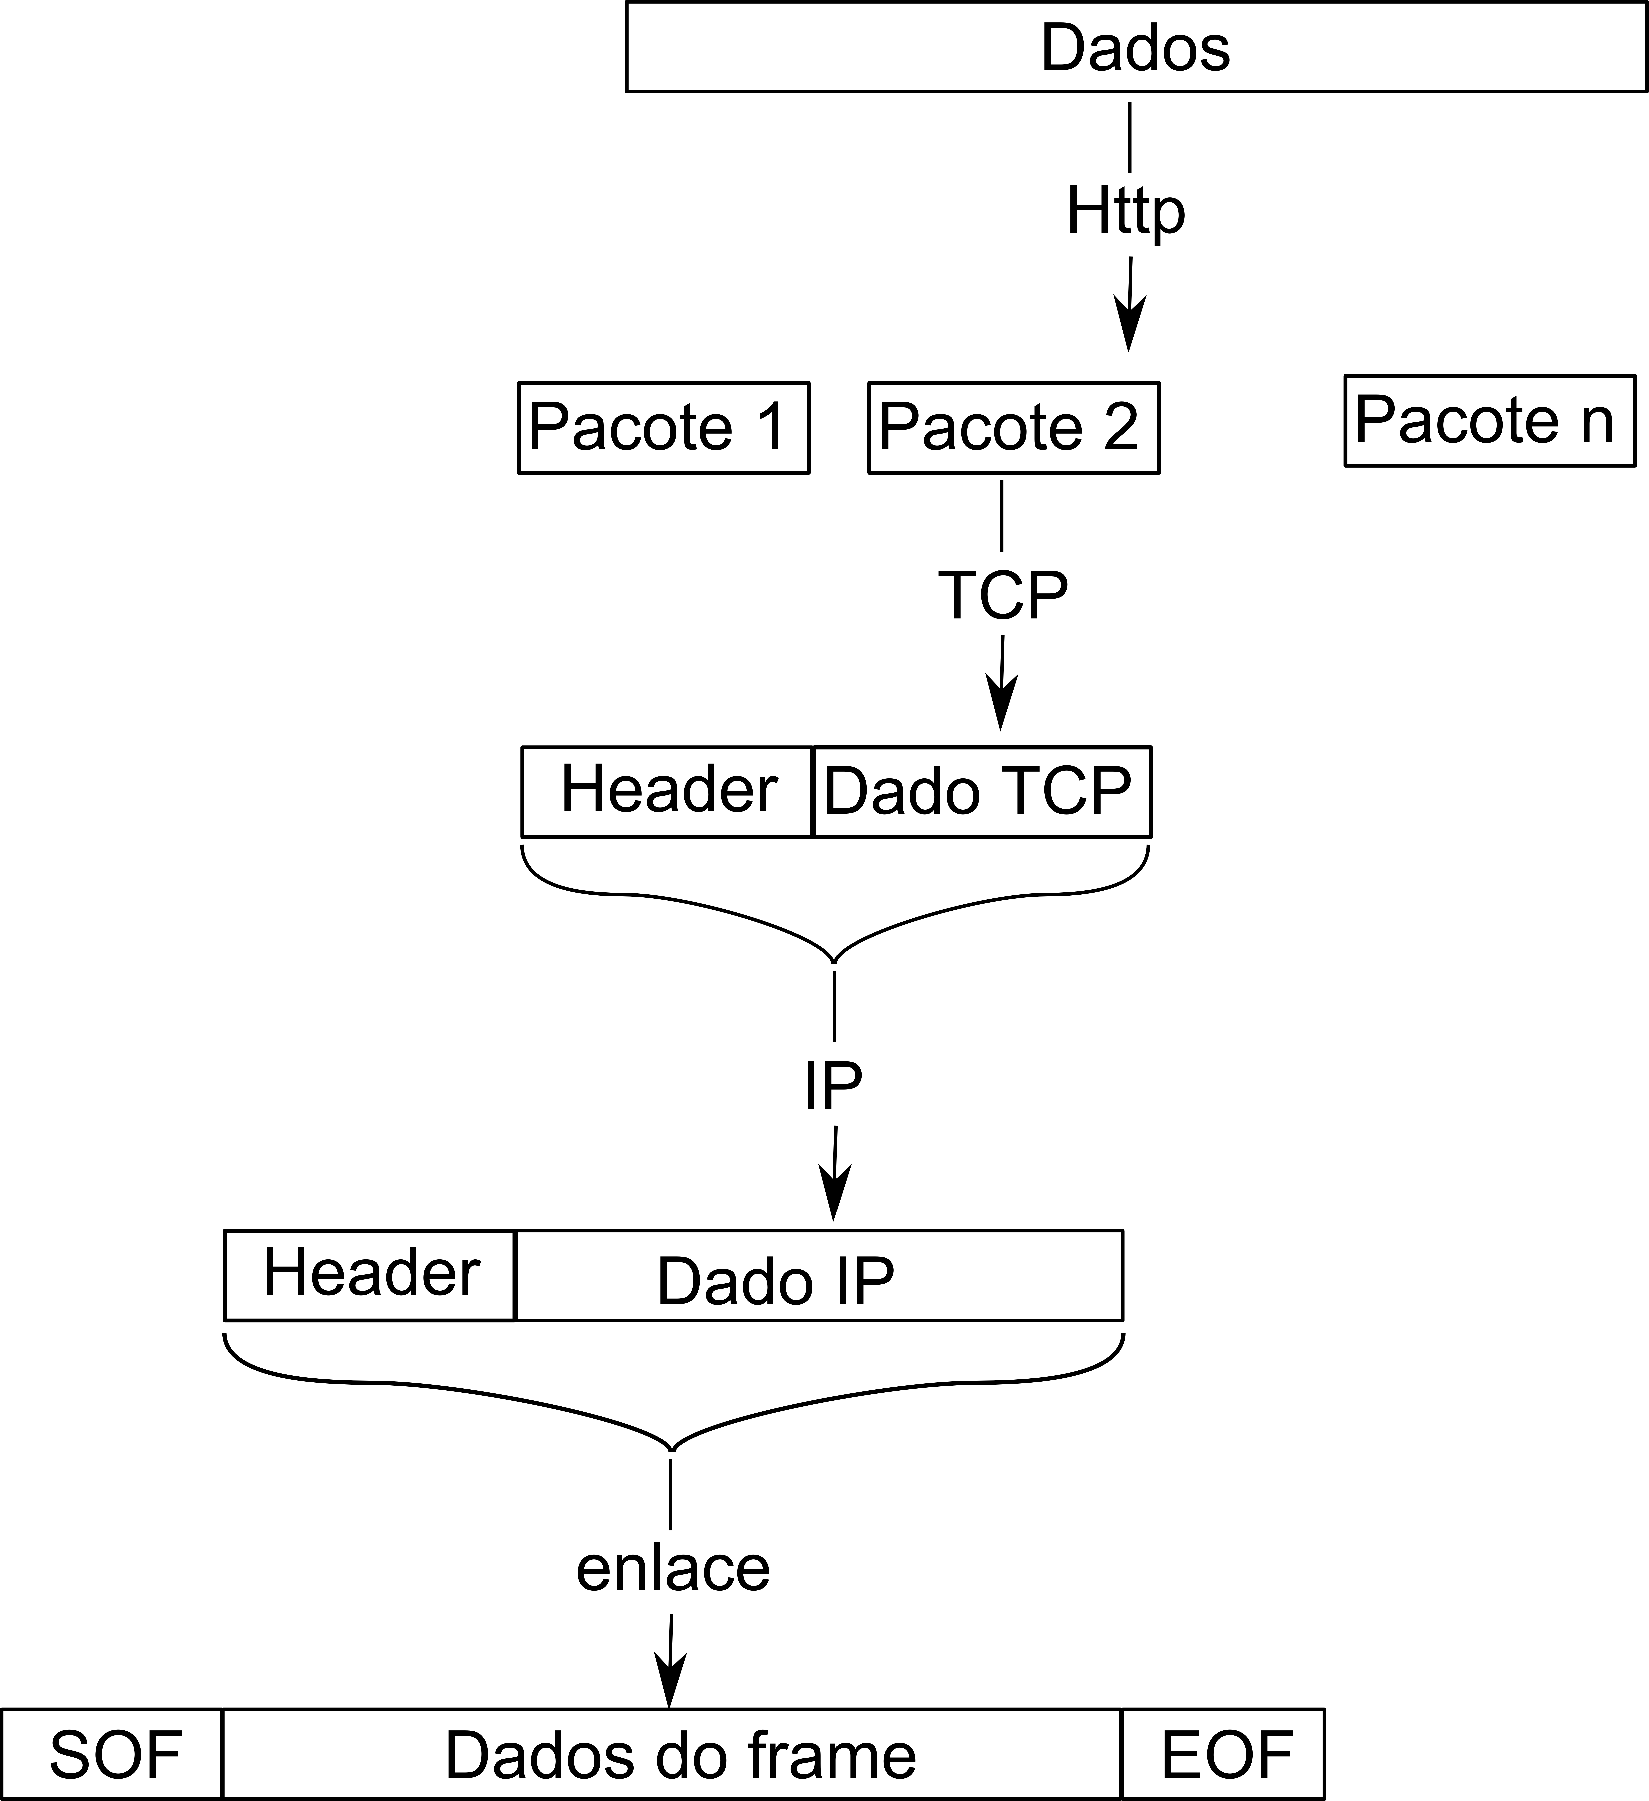
\includegraphics[width=\textwidth]{figuras/tcp-ip}
		\end{center}
		\caption{Encapsulamento da informação na pilha TCP/IP}
		\label{fig:tcp-ip}
	\end{figure}
